\documentclass[tikz,border=8pt]{standalone}
\usepackage{lmodern}
\usetikzlibrary{arrows.meta,angles,quotes,calc}
\definecolor{ink}{HTML}{183B4E}
\definecolor{teal}{HTML}{168C8C}
\definecolor{gold}{HTML}{D9982F}
\definecolor{softblue}{HTML}{EAF4F6}
\definecolor{softgold}{HTML}{FFF4D8}
\begin{document}
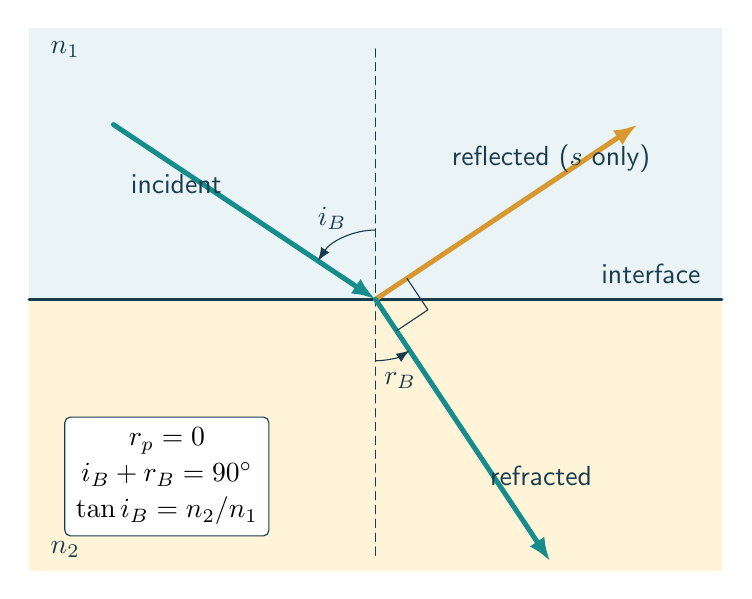
\begin{tikzpicture}[>=Latex,line cap=round,line join=round,font=\sffamily]
  \pgfmathsetmacro{\ib}{atan(1.5)}
  \pgfmathsetmacro{\rb}{90-\ib}
  \coordinate (O) at (0,0);
  \coordinate (N) at (0,3.25);
  \coordinate (D) at (0,-3.25);
  \coordinate (I) at ({-4*sin(\ib)},{4*cos(\ib)});
  \coordinate (R) at ({4*sin(\ib)},{4*cos(\ib)});
  \coordinate (T) at ({4*sin(\rb)},{-4*cos(\rb)});

  \fill[softblue] (-4.4,0) rectangle (4.4,3.45);
  \fill[softgold] (-4.4,-3.45) rectangle (4.4,0);
  \draw[ink,line width=1pt] (-4.4,0)--(4.4,0);
  \draw[ink,densely dashed] (D)--(N);
  \node[ink,anchor=south west] at (-4.25,2.95) {$n_1$};
  \node[ink,anchor=north west] at (-4.25,-2.95) {$n_2$};
  \node[ink,anchor=south east] at (4.25,0.08) {interface};

  \draw[teal,line width=1.8pt,-{Latex[length=3mm]}] (I)--(O);
  \draw[gold,line width=1.8pt,-{Latex[length=3mm]}] (O)--(R);
  \draw[teal,line width=1.8pt,-{Latex[length=3mm]}] (O)--(T);
  \node[ink,above left] at ($(I)!0.45!(O)$) {incident};
  \node[ink,above] at ($(O)!0.67!(R)$) {reflected ($s$ only)};
  \node[ink,below right] at ($(O)!0.60!(T)$) {refracted};

  \draw[ink,->] (0,.88) arc[start angle=90,end angle={90+\ib},radius=.88];
  \node[ink] at ({1.17*cos(90+\ib/2)},{1.17*sin(90+\ib/2)}) {$i_B$};
  \draw[ink,->] (0,-.78) arc[start angle=270,end angle={270+\rb},radius=.78];
  \node[ink] at ({1.08*cos(270+\rb/2)},{1.08*sin(270+\rb/2)}) {$r_B$};
  \pic[draw=ink,angle radius=4.8mm] {right angle=R--O--T};

  \node[draw=ink,fill=white,rounded corners=2pt,inner sep=4pt,align=center]
    at (-2.65,-2.25)
    {$r_p=0$\\[1pt]$i_B+r_B=90^\circ$\\[1pt]$\tan i_B=n_2/n_1$};

\end{tikzpicture}
\end{document}
